\documentclass[letterpaper,10pt]{article}
\usepackage[top=2cm, bottom=1.5cm, left=1cm, right=1cm]{geometry}
\usepackage{amsmath, amssymb, amsthm,graphicx,enumitem}
\usepackage{fancyhdr}
\pagestyle{fancy}

\lhead{\today}
\chead{MV Stats Assignment 3}
\rhead{Justin Hood}

\newcommand{\Z}{\mathbb{Z}}
\newcommand{\Q}{\mathbb{Q}}
\newcommand{\R}{\mathbb{R}}
\newcommand{\C}{\mathbb{C}}
\newtheorem{lem}{Lemma}

\begin{document}
\begin{description}
\item[3.2]\hfill \\
Consider,
\[X=\begin{bmatrix}
3 & 4\\6 & -2\\ 3 & 1
\end{bmatrix} \]
\begin{enumerate}[label=\alph*.]
\item To begin, we shall plot the scatter plot representation of this data in $p=2$ dimensions, along with the sample mean. We see the results in the plot below, with the data represented in blue, and the sample mean in red. The sample mean is computed as,
\[\bar{x}=\begin{bmatrix}
\frac{3+6+3}{3} & \frac{4-2+1}{3}
\end{bmatrix}=\begin{bmatrix}
4 & 1
\end{bmatrix} \]
\begin{center}
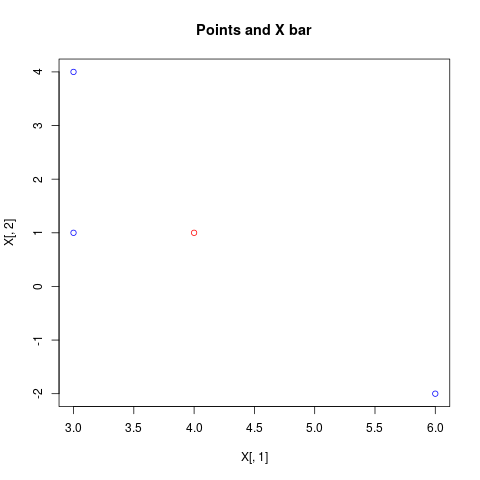
\includegraphics[scale=0.65]{32a.png}
\end{center}
We see that this point corresponds to the centroid of the triangle the points create, as desired.
\item Next, we will attempt a 3-d representation of the data along with the deviation vectors. First, we compute the deviation vectors as,
\[d_1=\begin{bmatrix}
3\\6\\3
\end{bmatrix}-\bar{x}_1\begin{bmatrix}
1\\1\\1
\end{bmatrix}=\begin{bmatrix}
3\\6\\3
\end{bmatrix}-\begin{bmatrix}
4\\4\\4
\end{bmatrix}=\begin{bmatrix}
-1\\2\\-1
\end{bmatrix} \]
Similarly,
\[d_1=\begin{bmatrix}
4\\-2\\1
\end{bmatrix}-\bar{x}_2\begin{bmatrix}
1\\1\\1
\end{bmatrix}=\begin{bmatrix}
4\\-2\\1
\end{bmatrix}-\begin{bmatrix}
1\\1\\1
\end{bmatrix}=\begin{bmatrix}
3\\-3\\0
\end{bmatrix}\]
These vectors (in red) along with the true data vectors (in blue) are found in the following plot,
\begin{center}
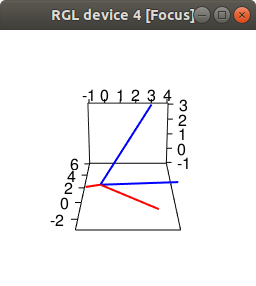
\includegraphics[scale=1]{32b.png}
\end{center}
It is difficult to visualize from this 2d representation, but we see that the deviation vectors are perpindicular to their corresponding sample mean, as desired.
\item We now compute,
\begin{align*}
|d_1| &= \sqrt{1+4+1}\\
&= \sqrt{6}\\
|d_2| &= \sqrt{9+9+0}\\
&=\sqrt{18}
\end{align*}
We now note that, 
\[\cos(\theta)=\frac{d_1'd_2}{|d_1||d_2|}=\frac{-9}{6\sqrt{3}}\approx-0.86603\]
We now consider,
\begin{align*}
d_1'd_1 &=\begin{bmatrix}
-1 & 2 & -1
\end{bmatrix}\begin{bmatrix}
-1 \\ 2 \\-1
\end{bmatrix}\\
&=6\\
&=3s_{11}\Rightarrow s_{11}=2
\end{align*}
Similarly,
\begin{align*}
d_2'd_2 &= \begin{bmatrix}
3 & -3 & 0
\end{bmatrix}\begin{bmatrix}
3\\-3\\0
\end{bmatrix}\\
&=18\\
&=3s_{22}\Rightarrow s_{22}=6\\
d_1'd_2 &= \begin{bmatrix}
-1 & 2 & -1
\end{bmatrix}\begin{bmatrix}
3\\-3\\0
\end{bmatrix}\\
&=-9\\
&=3s_{12}\Rightarrow s_{12}=-3
\end{align*}
We may now compute,
\[r_{12}=\frac{s_{12}}{\sqrt{s_{11}}\sqrt{s_{22}}}=\frac{-3}{\sqrt{2}\sqrt{6}}\approx -0.88603\]
Equal to the cosine of the angle from before. Thus,
\[S=\begin{bmatrix}
2 & -3\\
-3 & 6
\end{bmatrix} \]
\[R=\begin{bmatrix}
1 & \frac{-3}{\sqrt{2}\sqrt{6}}\\
\frac{-3}{\sqrt{2}\sqrt{6}} & 1
\end{bmatrix} \]
\end{enumerate}
\item[3.5b]\hfill \\
We again consider the $X$ matrix defined above. To compute the generalized sample variance, we first compute $S$ where,
\[S_{ik}=\frac{1}{n-1}\sum_{j=1}^n(x_{ji}-\bar{x}_i)(x_{jk}-\bar{x}_k)\]
Using, $R$, we find this matrix to be,
\[S=\begin{bmatrix}
3 & \frac{-9}{2}\\
\frac{-9}{2} & 9
\end{bmatrix} \]
The generalized sample variance is then,
\[|S|=3(9)-(\frac{-9}{2})^2=\frac{27}{4}=6.75\]
\item[3.9]\hfill\\
We consider the matrix,
\[X=\begin{bmatrix}
12 & 17 & 29\\
18 & 20 & 38\\
14 & 16 & 30\\
20 & 18 & 38\\
16 & 19 & 35
\end{bmatrix} \]
To begin, we compute the sample means as before,
\[\bar{x}=\begin{bmatrix}
16 & 18 & 34
\end{bmatrix}\]
We now compute the corrected data matrix as,
\[X-\textbf{1}\bar{x}'=\begin{bmatrix}
-4 & -1 & -5\\
2 & 2 & 4\\
-2 & -2 & -4\\
4 & 0 & 4\\
0 & 1 & 1
\end{bmatrix} \]
We note that again, column 3 is the sum of the previous two columns. Using this relation, we consider the $a$ vector, $[1,1,-1]$. As a test, in $R$ we compute,
\[(X-\textbf{1}\bar{x}')a=\begin{bmatrix}
0\\0\\0\\0\\0
\end{bmatrix}\]
Hence, we see that there is linear dependence as we suspected.\\
Next, we compute the sample covariance as before, using $R$, to obtain,
\[S=\begin{bmatrix}
10 & 3 & 13\\
3 & 2.5 & 5.5\\
13 & 5.5 & 18.5
\end{bmatrix} \]
Then,
\[|S|=160+48-208=0\]
As desired. We now compute,
\[Sa=\begin{bmatrix}
10 & 3 & 13\\
3 & 2.5 & 5.5\\
13 & 5.5 & 18.5
\end{bmatrix}\begin{bmatrix}
1\\1\\-1
\end{bmatrix}=\begin{bmatrix}
0\\0\\0
\end{bmatrix} \]
Thus, $a$ may be scaled to an eigenvalue. Finally, we note,
\begin{align*}
(n-1)Sa&=(X-\textbf{1}\bar{x}')'(X-\textbf{1}\bar{x}')a\\
&=(X-\textbf{1}\bar{x}')\textbf{0}\\
&=0
\end{align*}
Noting this, as well as the above compuation $Sa=0$, we see that for all $j$,
\[1(x_{j1}-\bar{x}_1)+1(x_{j2}-\bar{x}_2)-1(x_{j3}-\bar{x}_3)=0\]
From this, we concluide that the third variable is the sum of the first two.
\item[3.13]\hfill\\
Consider a data matrix $X$ and its correlation matrix $R$. Now consider a new matrix
$H$ where $H$ contains the standardized observations of $X$,
\[\eta_{jk}=\frac{x_{jk}-\bar{x}_{k}}{\sqrt{s_{kk}}}\]
We now consider, 
\[\bar{\eta}_k=\frac{\sum_{j=1}^n\eta_{jk}}{n}=\frac{\sum_{j=1}^n\frac{x_{jk}-\bar{x}_{k}}{\sqrt{s_{kk}}}}{n}=\frac{1}{n\sqrt{s_{kk}}}\sum_{j=1}^n x_{jk}-\bar{x}_{k}\]
We now note that the sum of $x_{jk}-\bar{x}_k$ will always be zero, and as such $\bar{\eta}_k=0,\ \forall k$. We now compute the elements of the covariance matrix,
\[s_{ik}=\frac{1}{n}\sum_{j=1}^n(\eta_{ji}-\bar{\eta}_i)(\eta{jk}-\bar{\eta}_k)=\frac{1}{n}\sum_{j=1}^n(\eta_{ji}-0)(\eta{jk}-0)\]
Substituting our definition of $\eta_{jk}$,
\[s_{ik}=\frac{1}{n}\sum_{j=1}^n(\frac{x_{ji}-\bar{x}_{i}}{\sqrt{s_{ii}}})(\frac{x_{jk}-\bar{x}_{k}}{\sqrt{s_{kk}}})=\frac{1}{\sqrt{s_{ii}}\sqrt{s_{kk}}}\frac{1}{n}\sum_{j=1}^n(x_{ji}-\bar{x}_i)(x_{jk}-\bar{x}_k)\]
Our traditional form of the covariance formula. Thus, we see that the standardized values have the same covariance as the original correlation matrix.
\item[3.14]\hfill\\
We consider the matrix,
\[X=\begin{bmatrix}
9 & 1\\5 & 3\\1 & 2
\end{bmatrix} \]
and the linear combinations of the matrix,
\begin{align*}
c'X &=\begin{bmatrix}
-1 & 2
\end{bmatrix}\begin{bmatrix}
X_1\\X_2
\end{bmatrix}=-X_1+2X_2\\
b'X&=\begin{bmatrix}
2 & 3
\end{bmatrix}\begin{bmatrix}
X_1\\X_2
\end{bmatrix}=2X_1+3X_2\\
\end{align*}
We begin by computing the sample means and variances for both $b$ and $c$ as follows.
\begin{align*}
b'x_1 &= 2x_{11}+3x_{12}\\
&=2(9)+3(1)\\
&=21\\
b'x_2 &= 2x_{21}+3x_{22}\\
&=2(5)+3(3)\\
&=19\\
b'x_3 &= 2x_{31}+3x_{32}\\
&=2(1)+3(2)\\
&=8\\
c'x_1 &=-1x_{11}+2x_{12}\\
&=-1(9)+2(1)\\
&=-7\\
c'x_2 &=-1x_{21}+2x_{22}\\
&=-1(5)+2(3)\\
&=1\\
c'x_3 &=-1x_{31}+2x_{32}\\
&=-1(1)+2(2)\\
&=3\\
\end{align*}
\[\bar{b}=\frac{21+19+8}{3}=16\]
\[Var(b)=\frac{(21-16)^2+(19-16)^2+(8-16)^2}{2}=49\]
\[\bar{c}=\frac{-7+1+3}{3}=-1\]
\[Var(c)=\frac{(-7+1)^2+(1+1)^2+(3+1)^2}{2}=28\]
Finally, the covariance becomes,
\[Cov(b,c)=\frac{(21-16)(-1+1)+(19-16)(1+1)+(8-16)(3+1)}{2}=-28\]
Next, we perform the same calculations using matrix algebra. We first compute the mean of each column of $X$ as,
\[\bar{x}=[5,2]\]
\[X_{adj}=X-\bar{x}\textbf{1}=\begin{bmatrix}
4 & -1\\0 & 1\\-4 & 0
\end{bmatrix} \]
Then, $S$ becomes,
\[S=\frac{1}{n-1}X_{adj}'X_{adj}=\begin{bmatrix}
16 & -2\\-2 & 1
\end{bmatrix} \]
We then use the results of (3-36) to compute the following,
\begin{align*}
b'\bar{x} &= 16\\
c'\bar{x} &= -1\\
b'Sb &= 49\\
c'Sc &= 28\\
b'Sc &= -28
\end{align*}
The same results as before, as desired.
\end{description}
\end{document}
